\documentclass{article}
\usepackage{graphicx}
\usepackage{CJKutf8}
\usepackage{algorithmic}
\usepackage{algorithm}
\usepackage{amsmath}
\usepackage{float}
\usepackage{xcolor}
\usepackage{listings}
\definecolor{dkgreen}{rgb}{0,0.6,0}
\definecolor{gray}{rgb}{0.5,0.5,0.5}
\definecolor{mauve}{rgb}{0.58,0,0.82}
\lstset{
	numberstyle=\footnotesize\color{black},
  	keywordstyle=\color{blue},
  	commentstyle=\color{dkgreen},
  	stringstyle=\color{mauve},
	language=python,
	numbers=left, 
	escapeinside=``, 
	basicstyle=\normalsize, tabsize=4,
	breaklines=true,
	backgroundcolor=\color{white},
	frame=shadowbox
}

\usepackage{lipsum}
\makeatletter
\newenvironment{breakablealgorithm}
{% \begin{breakablealgorithm}
	\begin{center}
		\refstepcounter{algorithm}% New algorithm
		\hrule height.8pt depth0pt \kern2pt% \@fs@pre for \@fs@ruled
		\renewcommand{\caption}[2][\relax]{% Make a new \caption
			{\raggedright\textbf{\ALG@name~\thealgorithm} ##2\par}%
			\ifx\relax##1\relax % #1 is \relax
			\addcontentsline{loa}{algorithm}{\protect\numberline{\thealgorithm}##2}%
			\else % #1 is not \relax
			\addcontentsline{loa}{algorithm}{\protect\numberline{\thealgorithm}##1}%
			\fi
			\kern2pt\hrule\kern2pt
		}
	}{% \end{breakablealgorithm}
		\kern2pt\hrule\relax% \@fs@post for \@fs@ruled
	\end{center}
}
\makeatother

\renewcommand{\algorithmicrequire}{\textbf{Input:}} 
\renewcommand{\algorithmicensure}{\textbf{Output:}}


\title{搜索算法:盲目搜索和启发式搜索}
\author{18308133 刘显彬}
\date{\today}
\begin{document}
\begin{CJK}{UTF8}{gbsn}	
		\maketitle
\section{实验原理}
	\subsection{双向搜索}
	\textbf{BFS:}宽度优先搜索是指,从起点处按照邻接点距离起点的次序进行搜索,直观上:搜索的点从起点处“一圈一圈”地往外延伸;如果把搜索点集看作是树,则是按点的深度按次序搜索。\\为了形式化说明:设该树的最大度为$b$,解节点的深度为$d$,称下一次需要探索的节点集为\textbf{边界},边界是一个\textbf{先进先出的队列}结构,则BFS每次将探索到(但在此之前还没探索过)的节点放入边界末端,直接探索到目标节点。\\ \\
		\textbf{复杂度}:BFS的空间消耗用于:边界的存储以及节点访问状态的存储:前者最坏情况下需要存储深度为d的所有节点,空间复杂度为$O(b^d)$;后者则需要存储深度小于等于d的所有节点状态,空间复杂度为$O(b^{d+1})=O(b^d)$,因此总复杂度为$O(b^d)$;时间复杂度等于要访问的点数:即$O(b^d);$
		\\ \\
	\textbf{双向搜索:}双向搜索是BFS的进化版:指从起点和终点同时进行BFS搜索,直到这两支路径访问了同一个点,则说明找到了一个解,因为BFS是探索节点深度不断加深的搜索,所以解是最短路径解(如果邻接节点的距离一样的话),所以双向搜索也是最短路径解。对任意一支BFS树,找到解后其深度均为$d/2$,因此其空间复杂度为:$2O(b^{d/2+1})=O(b^{d/2})$,时间复杂度依赖于访问的点数,因此和空间复杂度一致。可见双向搜索是优于单纯的BFS。\\
	\\
	\textbf{环检测}:BFS中,首先访问到一个点的路径$P_1$总是最短的,因此,其他路径$P_n$访问到该点后,总是更长的,因此路径$Pn$不必再从此处延伸。
	
	\subsection{A*搜索}
		\textbf{启发式搜索}:上面的两种搜索并没有利用边界上点的信息,也就是没有对它们进行评估:哪个更有可能到达终点,这类搜索算法也称作为无信息/盲目搜索。而在启发式搜索中,会对边界的点进行评估,这种利用额外的知识的评估方法也称为\textbf{启发式函数}。
		\\ \\
		\textbf{A*搜索}:定义实际代价函数$g(n)$:到达点$n$时的实际代价;以及启发式函数$h(n)$,在对\textbf{边界}进行探索时,将优先会探索使$f(n)=g(n)+h(n)$最小的点,因为很可能是一个更$promising$的方向。
		\\ \\ 
		\textbf{可采纳性}:$\forall n, h(n)<h^*(n)$时,也就是说对点n的评估代价比真实代价都要小。满足可采纳性时:我们将会低估最优解的代价(记为$C^*$),根据$A^*$搜索的原理,评估代价小于$C^*$的点都会被访问,也就保证了最优解会被选中,也就是说:可采纳性意味着最优性。\\
		\textbf{一致性}:$\forall n_1, n_2, h(n_1)\le g(n_1\rightarrow n_2)+h(n_2)$,直观上讲:“两边之和大于第三边”:直接对$n_1$的评估代价要小于先从$n_1\rightarrow n_2$的代价加上对$n_2$的评估代价。一致性保证了一个点被最先一条路径探索到时,该路径一定是代价最小的:设一条路径上依次的点为$n_i$
		\begin{itemize}
			\item $f(n_i)=g(n_i)+h(n_i)\le g(n_i)+g(n_i\rightarrow n_{i+1})+h(n_{i+1})=f(n_{i+1})$,也就是$f(n_i)$是非递减的。
			\item 以上保证了更小f值的点会先被探索,对于任意终点n,首个访问到它的路径,其f(n)比其他路径到该点都要小,而对于终点h(n)=0,因此实际成本g(n)也是最小的。
		\end{itemize}
		因此,满足可采纳性和一致性的启发式函数的$A^*$搜索通过环检测剪枝后的解是最优。
\section{伪代码}
	\subsection{双向搜索}
	\begin{breakablealgorithm}
	\caption{biSearch(Problem, s, e)}\label{1}
	\begin{algorithmic}[1]
		\REQUIRE Problem Tree, s : start point, e : end point
		\ENSURE $MinPath(s\rightarrow e)$ or failure
		
		\STATE $bs \gets \o \cup s$ // 从s出发的边界
		\STATE $be \gets \o \cup e$
		\WHILE {$not\ empty(bs, be)$}
		\STATE 依次扩展s,e为起点的边界
			\FORALL{$node \in bs$}
			\FORALL{$action \in Problem.action(node)$}	
				\STATE $newnode \gets Node(Problem, node, action);$
				\IF{$newNode.pos \in Problem.VisitFrom(e)$}
					\STATE //如果该点已经在另一侧被访问,说明两侧联通(有解)
					\STATE $result \gets newnode.Path \cup Problem.PathFromE(newnode)$
					\STATE return result
				\ELSIF{$Problem.notVisited(newnode)$}
				\STATE $bs \gets bs \cup \{newnode\}$
				\ENDIF
			\ENDFOR
			\ENDFOR
			\STATE // 和上面相同,处理从终点出发的BFS
			\FORALL{$node \in be$}
			\FORALL{$action \in Problem.action(node)$}
				\STATE $newnode \gets Node(Problem, node, action);$
				\IF{$newNode \in Problem.VisitFrom(s)$}
					\STATE $result \gets node.Path \cup \{newnode\}$
					\STATE return result
				\ELSIF{$Problem.notVisited(newnode)$}
				\STATE $be \gets be \cup \{newnode\}$
				\ENDIF
			\ENDFOR
			\ENDFOR
		\ENDWHILE
		\STATE return failure
	\end{algorithmic}
	\end{breakablealgorithm}

	\subsection{A*搜索}
	\begin{breakablealgorithm}
		\caption{AstartSearch(Problem)}\label{2}
		\begin{algorithmic}[1]
			\REQUIRE Problem Tree
			\ENSURE PATH with A* or failure
			
			\STATE $b\gets \{Problem.start\}$
			\WHILE{notEmpty(b)}
				\STATE $node \gets b.popHead()$ //在队列头弹出一个节点
				\FORALL{$action \in Problem.Action(node)$}
					\STATE $new \gets Node(node, action)$
					\IF{$new \in Problem.Visited$}
					\STATE //环检测剪枝
					\STATE continue
					\ELSIF {new is Problem.end}
					\STATE return new.Path
					\ENDIF
					\STATE //插入边界,并计算f值,然后对边界排序
					\STATE $new.h \gets Problem.h(new)$
					\STATE $new.f\gets new.cost+new.h$
					\STATE $bs \gets bs \cup \{new\}$
					\STATE sort bs with element.f, Desc
					\ENDFOR
			\ENDWHILE
			\STATE return failure
		\end{algorithmic}
	\end{breakablealgorithm}
\section{关键代码分析}
	\subsection{双向搜索}
	\subsubsection{搜索过程}
	下面展示的是,双向BFS中其中一支扩展边界的过程,代码中变量$Ss,Se$分别代表了两个方向(fromStart、fromEnd)的已访问节点集合,主要思路就是取出边界中所有节点并探索它们的邻居,利用$Ss$进行环检测,利用$Se$两个分支是否汇合。在文件处理中,将节点的状态存在一个numpy.array中,其中0:有路,1:墙,2:起点,3:终点;第10行的state就是以上取值的一种。
	\begin{lstlisting}
while(len(fromStart)!= 0 or (len(fromEnd))!= 0):
	# start from Start set
    Ls = len(fromStart) # to calculate how many node should be visited
    while Ls != 0:
		Ls -= 1
		StartCnt += 1
		if (found): break
		cur = fromStart.pop(0)
		for son, action in self.neigh(cur):
			state = self.map[son[0],son[1]]
			if (state == 1) or (state == 2): continue
			son = tuple(son)
	        if son in Se:
           		Ss[son] = int(action)
		        meet = son	#meet at this node
				found = 1
				break                   
			elif son in Ss:
				# cirle checking -- cut
                continue
            else:
				# a new node
				Ss[son] = int(action)
				fromStart.append(son)

	\end{lstlisting}
	\subsubsection{回溯建路}
	回溯建路也是相似的两部分:$start\rightarrow meet\ node\rightarrow end$,这里选前一部分来分析:在相遇点$meet$处往前回溯,根据坐标$meet$映射到该节点的信息:$action$来恢复它的父亲节点的坐标,重复该过程直到访问到start。此处规定了行动序列$\{1,2,3,4\}$表示由父亲节点向:左右下上行动而来。第6行处的$a2char$是一个由行动序列到表现字符的映射表(如$1:\  '\rightarrow'$,这只是在表达路径时输出的字符)
	\begin{lstlisting}
def buildPath(self, meet, Ss, Se):
    Paths, Pathe = [], []
	endS = endE = meet
    while endS != self.s:
        action = Ss[endS]
        Paths.append(self.a2char[action])
        endS = tuple(np.array(endS)-self.a2pos[action])
		\end{lstlisting}
	\subsection{$A^*$搜索}
		\subsubsection{搜索过程}
		变量声明:State是已访问点的集合(实际上是python中的‘字典’,由坐标映射到Node节点),用于回溯建路以及环路检测,boundry表示边界,是一个按元素的‘f’值排序的最小堆,支持插入元素(insert)和弹出最小值(pop)
		\begin{lstlisting}
root = Node(self.s)
State = {self.s:root}
boundry = MinHeap([root], key=lambda node:node.f)
		\end{lstlisting}
		下面是搜索过程:具体过程与双向搜索的分析类似:不断弹出边界中(f值)的最小节点,探索其子节点:(1)是否是终点(第8行)(2)是否是路,然后判断是否已经探索过,没有则计算其f值并加入边界
		\begin{lstlisting}
while len(boundry)!= 0:
    if (found): break
    cur = boundry.pop()
    for son, action in self.neigh(cur.pos):
        son = tuple(son)
        action = int(action)
        pstate = self.map[son[0],son[1]]
        if pstate == 3:
            last = son
            found = 1
            State[son]=Node(son, action, cur)
            break
        if pstate == 0:
            if tuple(son) in State:
                # cut
                continue
            else:
                Cnt += 1
                newnode = Node(son, action, cur)
                newnode.h = self.h(newnode)
                newnode.calcf()
                State[son]=newnode
                # sort Boundry
                boundry.insert(newnode)
		\end{lstlisting}
		\subsubsection{回溯建路}
			这一部分与双向搜索相似。
		\subsubsection{h(n)的选取}
			这次迷宫实验的启发式函数我设置为:距离终点的街区距离。\\
			\begin{lstlisting}
def h(self, node:Node):
	return abs(node.x-self.e[0])+abs(node.y-self.e[1])
			\end{lstlisting}
			\textbf{可采纳性:}每前进一格,当前的节点的h值最多减1,到达终点的实际代价也最多只能减少1,因此由终点递推回起点,总有h值总是低估实际代价,即$h(n)\le h^*(n)$\\
			\textbf{一致性:}假设每一步都往终点靠近,$h(n_i)-h(n_{i+1})=1$,而实际代价$g(n_i\rightarrow n_{i+1})=1$,所以$h(n_i) = g(n_i\rightarrow n_{i+1})+h(n_{i+1})$;而如果远离终点,$h(n_{i+1})>h(n_i)$。综上所述:$h(n_i) \le g(n_i\rightarrow n_{i+1})+h(n_{i+1})$
\section{实验结果分析}
	迷宫如下,其中0表示路,1表示墙,S、E分别表示起止点\\
	\begin{figure}[H]
		\centering
		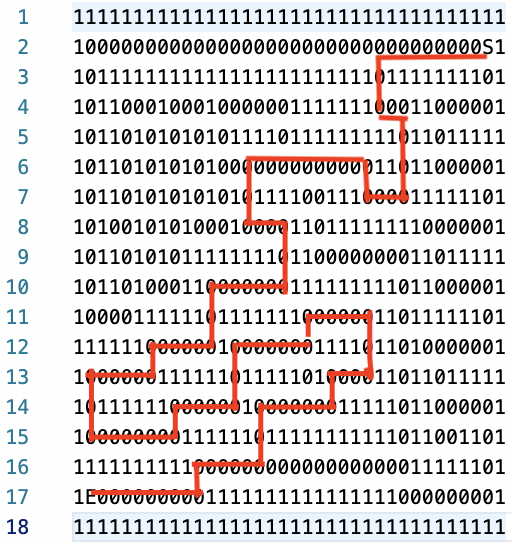
\includegraphics[scale=0.8]{fig/2}
	\end{figure}

	双向搜索结果如下:\\
	\begin{figure}[H]
	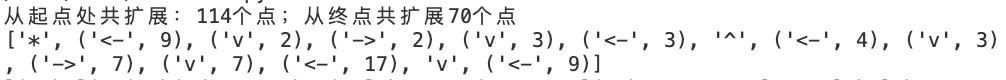
\includegraphics[scale=0.8]{fig/1}	
	\end{figure}

	$A^*$搜索结果如下:
	\begin{figure}[H]
	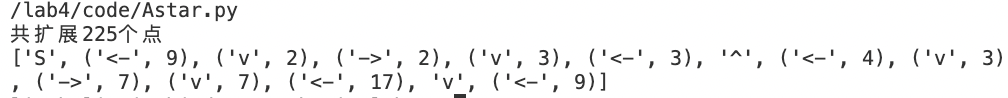
\includegraphics[scale=0.8]{fig/3}
	\end{figure}
	
	将$A^*$稍微修改一下$h(n)=0$,就可以得到BFS,运行结果如下:
	\begin{figure}[H]
	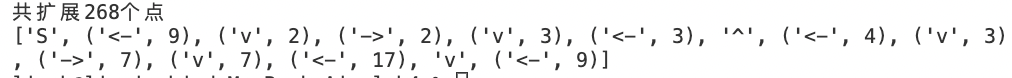
\includegraphics[scale=0.8,trim=0 5 0 0, clip]{fig/4}	
	\end{figure}
	
	可见,相比于单纯的BFS,双向BFS和$A^*$搜索都有效地减少了访问的节点,其中双向BFS在两侧同时扩展,更快地让两个分支碰面,而$A^*$利用了位置信息权衡了更有可能的方向,因此也避开了部分不需要探索的节点。
\section{思考题}
	\subsection{比较上述策略的性能}
	\textbf{完备性}:两个算法都是BFS的升级版,自距离/代价从小到大扩充边界,在有解且空间足够的情况下,它们都能找到解。\\
	\textbf{最优性}:BFS找到的解总是最优的,因为BFS总是从最短路径到达目标,双向BFS只是加速了这个过程:从起点和终点同时出发;而$A^*$则是在一致性的保护下,在经过了环检测的剪枝后也保留了最优性。\\ \\
	\textbf{时间\&空间复杂度}:时间和空间复杂度总是一致的:都依赖于它们访问过了的节点数:\\ \textbf{双向搜索
}中,将BFS中的指数复杂度打了5折,可以从上面的实验结果看出来:双向BFS确实大大减少了需要访问的点,而这种减少几乎可以说是必然的,直观上理解就是:从起点终点共同出发相遇时间总比一个人出发的时间要短一半。而且该搜索是稳定的,最好、最坏、平均意义下,复杂度相差不大。\\ \\
	\textbf{$A^*$搜索}利用了额外的知识作为扩展边界的次序依据,所以复杂度的分析与启发函数的优劣有着密切关系,好的启发函数可以快速确定前往终点的大方向,从而能够减少大量的不必要探索,最好的情况下,总是能找到准确的方向,因此最好的情况下可以复杂度为$O(d)$,但最坏情况下,就会退化成BFS。
	因此:在完备性和最优性方面,二者是等价的;它们的主要不同在于时间空间复杂度,双向搜索必然是指数复杂度,但要远优于BFS,而$A^*$在有好的知识背景时,很可能会"出奇制胜",跳出指数复杂度;反之,则很可能会退化为$O(b^d)$。
	
	\subsection{思考不同搜索策略的优缺点以及他们的使用场景。}
	对于与BFS相关的盲目搜索(BFS、双向BFS、一致代价):它们总是能保证完备性和最优性,但时间和空间上总是会陷入指数复杂度,对于设备内存不足的情况下,并非是最好的选择。但需要找到\textbf{最优解}的情况下,是很好的选择。\\
	而与DFS则相反,它有着优秀的线性空间复杂度优势$O(bm)$,但是时间上仍然是指数复杂度,而且\textbf{不能保证在有限的时间能找到解,找到解时也未必是最优的}。所以如果问题本身内存有限的情况下,DFS可能是更好的选择。\\
	而DFS的延伸:迭代加深DFS算法结合了DFS和BFS的优势,能保证空间复杂度不过大,同时保证了完备性,在仅关注是否找到解的情况下,这个算法是更好的选择。但是\textbf{未必能保证解的最优性}(除非用额外的开销,将深度限制改为成本限制)。\\ \\
	而启发式搜索在通常情况下比以上的盲目搜索都要好,因为有良好的先验知识做代价评估的情况下,往往能指导路径往更好的方向延伸,因此可以将以上时间的指数复杂度,大大下降,是一种更高效的方法。但性能非常依赖启发式函数的选择。
	
\end{CJK}
\end{document}








